% 
% Practica ICO - Smart Player
% ------------------
% Ingeniería del Conocimento
% Universidad de Granada
% 
% Autor:
% - María Carrasco Rodríguez
% - Francisco Manuel Herrero Pérez
% 

\documentclass[a4paper,12pt,oneside]{book}
\usepackage[spanish]{babel}
\usepackage{graphicx}
\usepackage{ucs}
\usepackage{listings}
\usepackage[utf8]{inputenc}
\usepackage{amsfonts}
\usepackage{amssymb}
\usepackage{hyperref}
\usepackage{url}
\usepackage{multirow}
\usepackage{listings}  
\lstset{language=Python,commentstyle=\emph}
\usepackage{color} 
\usepackage{colortbl}
\hypersetup{linkbordercolor= 1 0.8 0.8}
\usepackage{phdthesis}
\usepackage{times}
\usepackage{setspace}
% \onehalfspacing
\renewcommand{\baselinestretch}{1.5}
%\doublespacing

% opening
\title{Jugador Inteligente}
\author{María Carrasco Rodríguez \\
  Francisco Manuel Herrero Pérez}
\date{Curso 2009/10}
\parskip = 7 pt

\makeindex

\begin{document}
\begin{titlepage}
  \parskip = 6pt
  \null\vfil
  \hrule height 2pt
  \begin{center}
    \huge \textsf{\emph{ BattleTech}
      \\ \textbf{ Jugador Inteligente }}
    % \large \textit{\@subtitle}
  \end{center}
  \hrule height 2pt

  \begin{center}
    \large 
    María Carrasco Rodríguez \par 
    Francisco Manuel Herrero Pérez \par
    \vskip 15pt
    \hrule height 0.5pt
    \vskip 20pt
  \end{center}
  \begin{center}
    \small
    % \sffamily Universidad de Granada \par \vskip 1pt
    \sffamily Ingeniería del Conocimiento \par \vskip 1pt
    \footnotesize 
    \emph{Curso 09/10} \par
  \end{center}

  \vfil\null
\end{titlepage}


\tableofcontents

\pagebreak

\chapter{Introducción}
{\bf BattleTech} es un juego de combates entre enormes máquinas de
aspecto humanoide llamados {\it BattleMechs} (o más brevemente
llamados Mechs). \\
\begin{figure}[!h]
  \centering
  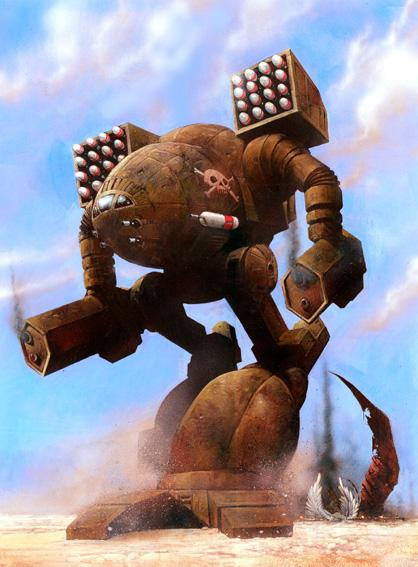
\includegraphics[width=7cm]{images/mech_super.jpg}
\end{figure}

Este juego fue diseñado por la compañía americana {\it FASA}, que
debido al gran éxito obtenido, ha ido creciendo hasta el infinito con
diversas aplicaciones.
En España, lo primero que se comercializó fué la trilogía de novelas
El sol y la espada, en la que {\it Michael A. Stackpole} desarrolla las
líneas argumentales básicas del universo que sirve de fondo para el
juego. Posteriormente, se editó el juego de tablero, la primera y
segunda versiones de las reglas del juego de rol, seguidos de
distintos accesorios (módulos, ampliaciones, figuras a escala, etc).\\

El juego trata del enfrentamiento por la supremacía entre cinco
unidades políticas herederas de un antiguo gran imperio -la Liga
Estelar-, que se extendía hasta los 300 años-luz de la Tierra. Tras
el derrumbe de la Liga, comienzan las Guerras de Sucesión entre las
Grandes Casas (las familias que rigen cada una de las unidades
políticas). Estas guerras acaban por destruir los medios de producción
de bienes, con lo que tras 300 años de guerra continuada, la economía
se basa en el saqueo sistemático para mantener la capacidad bélica de
los diversos ejércitos.\\


La acción principal de las novelas tiene lugar en el periodo
comprendido entre el 3027 y el 3058, en el que Hanse Davion, Principe
de la Federación de Soles, logra firmar una alianza con la
Mancomunidad de Lira para someter al resto de naciones y reinstaurar
la Liga Estelar. Esto da lugar a una serie de enfrentamientos
políticos y militares a gran escala que dan un buen transfondo al
juego de rol.\\


El juego -tanto en tablero como en rol- se basa en las unidades
militares de las Grandes Casas, compuestas por robots de 20 metros de
altura (Mechs), cada uno con más armas encima que pinchos tiene un
puercoespín. Como la ciencia ha decaido a un nivel similar al del
siglo XXII, estos están cayéndose a pedazos, pero aún así son capaces
de destrozar una ciudad sin esfuerzo. Aunque parezca un poco tonto eso
de llevar un robot por un tablero disparando a otros robots, es
divertidísimo. Si además lo incluyes en una campaña de un juego de
rol, puedes acabar por olvidarte de los otros vicios.


\section{Descripción del Problema}
\begin{quote}
  {\it En la practica se ha de diseñar
    y desarrollar un prototipo de
    Jugador Inteligente. }
\end{quote}

Nuestro objetivo es crear un jugador inteligente que sea capaz de
dirigir a los BattleMechs. Para ello debe decidir la acción a
realizar en cada momento por ellos. Nuestro problema se restringe
únicamente a controlar a los Mechs, aunque existan muchos otros tipos
de vehículos en los combates - BattleMech, vehículo, Pelotón de
infantería o Punta o Escuadra de armaduras de combate -.

\subsection{BattleMechs}
Titanes humanoides de metal de 12 metros de altura cubiertos con
láseres, cañones automáticos y docenas de otras armas letales; poder
suficiente para arrasar manzanas enteras de edificios. 

\subsection{Mapas}

En Battletech las partidas se juegan en mapas divididos en áreas de
seis lados llamadas hexágonos, las cuales regulan el movimiento y el
combate entre varias unidades. Los mapas pueden tener bosques, ríos,
lagos, montañas y más.

\subsection{Secuencia de Juego}

Una partida de Battletech consiste en una serie de turnos. Durante
cada turno todas las unidades en el mapa tienen la oportunidad de
moverse y disparar sus armas. Cada turno consiste en varios
segmentos de tiempo más pequeños, llamados fases.\\

Durante cada fase, los jugadores pueden escoger un tipo de acción,
cada turno incluye las correspondientes fases, que se desarrollan en
el orden siguiente:
\begin{enumerate}
\item Fase de Movimiento
\item Fase de Reacción
\item Fase de Ataque con Armas
\item Fase de Ataque Físicos
\item Fase de Final de Turno
\end{enumerate}

\subsubsection{ Fase de Movimiento }
El jugador que ha perdido la iniciativa mueve primero. El jugador que
ganó la iniciativa mueve entonces. El movimiento se alterna entre los
bandos hasta que todas las unidades se hayan movido. \\

Las unidades de Battletech cambian de posición y ubicación
en el mapa realizando uno de los distintos movimientos. Durante la
Fase de Movimiento de cada turno los jugadores deben escoger un modo
de movimiento, para los Mechs las opciones son andar, correr o saltar.

\subsubsection{ Fase de Reacción }
Fase posterior al movimiento que permite a los mechs de girar el
torso. Sólo se permite un movimiento de giro, por lo que podremos
girar a la derecha, a la izquierda o permanecer igual.

\subsubsection{ Fase de Ataque con Armas } 
Fase en la que los jugadores, por orden de iniciativa, pueden abrir
fuego con la artilleria de sus mechs. El Mech elegirá las armas que
disparara, dentro de las que dispone en su arsenal, y sobre qué
enemigo usarlas.

\subsubsection{ Fase de Ataque Físicos }
Fase en la que se presenta una nueva opción la opción de realizar daño
físico a otros Mech, y es la última opción de hacerles daño dentro del
turno en el que nos encontramos.
El ataque físico consistirá en realizar un impacto físico, con algún
garrote/arma o extremidad del robot.

\subsubsection{Fase  de Final de Turno }
Fase en la que los jugadores pueden determinar acciones especiales como
tirar algún garrote o munición al suelo o apagar o encender radiadores.

\subsection {Objetivo}
Nuestro objetivo principal en el juego será acabar con todos los
jugadores que haya en el tablero, exceptuando al nuestro. Para ello,
debemos destruir una a una el resto de las unidades que participan en
el juego.


\section {Abstracción del Problema}

Para resolver nuestro problema podemos ver al jugador inteligente como
un {\it ente}, que percibe el universo a través de un conjunto
entradas - que nos indican el estado actual del juego -. Este ente
debe ser capaz de escoger una acción a realizar.\\

Pero, ¿Cómo escoger cual de entre todas las posibles acciones a
realizar? La respuesta es bastante subjetiva, ya dependerá de la
estrategia a seguir. Según la escogida, se obtendrá un resultado mejor
o peor, pero también depende del caso concreto que estemos estudiando,
ya que si cambiamos ciertos parametros de nuestro universo, otra
estrategia puede resultar más favorable.\\

A la hora de decidir sobre qué estrategia seguir, se debe de tener en
cuenta que tanto la {\bf experiencia} adquirida tras años de juego y
el {\bf conocimiento} de las reglas del mismo, son puntos críticos a
la hora de maxímizar nuestro rendimiento.

Nuestro ente se mueve en un espacio temporal discreto, el juego se
divide por turnos y estos a su vez, se ve dividido en segmentos más
pequeños a los que llamaremos fases. Cada fase se utiliza para
realizar una acción determinada, y según la acción que queramos
realizar seguiremos una manera de razonar distinta según los objetivos
que queramos conseguir. Veamos entonces cada una de las fases.

\subsection{Fase de Movimiento}
\subsection{Fase de Reacción}
\subsection{Fase de Ataque con Armas}
\subsection{Fase de Ataque Físico}
\subsection{Fase de Final de turno}



\chapter{Modelo Teórico}
La inteligencia artificial, {\bf IA}, es una disciplina relativamente
nueva, la cual es considerada como una gran desconocida y una de las
que más interés profano despierta. Pero, {¿qué es realmente la IA?}
Aunque existen muchas definiciones, podemos resumirlas en {\it
  ``desarrollar sistemas que piensen y actúen racionalmente''}.\\

También hemos encontrado otras definiciones que resultan interesantes:
\begin{itemize}
\item {\it `` The exciting new effort to make computers think ... machines
    with minds, in the full literal sense.''} (Haugeland, 1985)\\
\item {\it `` The art of creating machines that perform functions that
    require intelligence shen permormed by people''} (kurzweil, 1990)\\
\item {\it `` The study of how to make computers do things at which, at the
    moment people are better''} (Rich and Knight, 1991)\\
\end{itemize}
En la IA se encuentra un paradigma conocido como {\it ``paradigma de
  agentes''}, que aborda el desarrollo de entidades que puedan actuar
de forma autómata y razonada. Si retomamos la definición dada
anteriormente donde se consideraba a la IA como un medio para el
desarrollo de sistemas que piensen y actúen racionalmente, podemos
pensar que la IA, en su conjunto, trata realmente de construir
precisamente dichas entidades autónomas e inteligentes.
\begin{quote}
  ``Los agentes constituyen el próximo avance más significativo en el
  desarrollo de sistemas y pueden ser considerados como la nueva
  revolución en el software.''
  Dr. Nicholas Jennings
\end{quote}

\section{Agente Inteligente}
Un agente inteligente, es una entidad capaz de percibir su entorno,
procesar tales percepciones y responder o actuar en su entorno de
manera racional, es decir, de manera correcta y tendiendo a maximizar
un resultado esperado.\\

En este contexto la racionalidad es la característica que posee una
elección de ser correcta, más específicamente, de tender a maximizar
un resultado esperado. Este concepto de racionalidad es más general y
por ello más adecuado que inteligencia (la cual sugiere entendimiento)
para describir el comportamiento de los agentes inteligentes. Por este
motivo es mayor el consenso en llamarlos {\it agentes racionales}.\\

Nuestro {\bf jugador inteligente} se corresponde con un {\bf agente racional}, y
por lo tanto debe poseer las características:
\begin{itemize}
\item {\bf Reactivo.} El jugador podrá responder a cambios en el
  entorno en el que se encuentra situado. Estos cambios se le indican
  al jugador mediante los ficheros, que en cada fase de la partida el
  jugador debe leer para obtener toda la información necesaria.
\item {\bf Pro-activo.} El jugador debe ser capaz de intentar cumplir
  sus planes u objetivos. Su objetivo final será destruir a el resto
  de los jugadores.
\item {\bf Autonomía.} Nuestro agente actuará sin intervención de
  ningún usuario externo a nuestro programa. Por tanto tiene control
  total sobre sus acciones y estados internos.
\end{itemize}

\begin{figure}[!h]
  \centering
  \includegraphics[width=12.4cm]{images/funcion.png}
  \caption{Esquema de funcionamiento.}
\end{figure}
Hemos de diferenciar nuestro sistema de los sistemas Multi-Agente
(SMA). Éstos son grupos de agentes que interaccionan entre sí para
conseguir objetivos comunes, pero en nuestro entorno los distintos
jugadores no se comunican entre sí - no tienen conducta social-. Si
tuvieramos esto en cuenta, aumentaría la complejidad en el
desarrollo.\\

Nuestro agente es {\it basado en metas}. Estas ayudan a decidir las acciones
correctas en cada momento. En nuestro juego, el agente o jugador
escoge un objetivo, en base al cual toma sus decisiones. Por tanto, no
basta con conocer el entorno, sino además es necesario determinar las
acciones a seguir que permitan alcanzar la meta. Elegir las acciones
correctas varia en complejidad.
\begin{itemize}
\item {\it Búsqueda}
\item {\it Planificación}
\end{itemize}
\begin{figure}[!h]
  \centering
  \includegraphics[width=13.5cm]{images/meta2.png}
  \caption{Agente basado en metas.}
\end{figure}

\section{Ambientes}
Existen diferentes tipos de ambientes:
\begin{itemize}
\item {\bf Accesibles y no accesibles.} En nuestro caso se trata de un
  ambiente accesible, ya que el agente tiene acceso al estado total
  del ambiente.
\item {\bf Deterministas y no deterministas.} Depende de si el estado
  siguiente se determina a partir del estado y las acciones elegidas
  por el agente.
\item {\bf Episódicos y no episódicos.} En ambientes episódicos, como
  es nuestro caso, la experiencia del agente se divide en
  ``episodios''- o fases-. Cada episodio consta de un agente que
  percibe y actúa.
\item {\bf Estáticos y dinámicos.} Si el abiente cambia mientras un
  agente toma una acción a seguir, entonces se dice que el ambiente es
  ``dinámico''. Pero en nuestro caso tratamos con ambientes {\it
    estáticos}, puesto que no se tiene que observar y pensar al mismo tiempo.
\item {\bf Discretos y continuos.} Si existe una cantidad limitada de
  percepciones y acciones distintas y discernibles, se dice que el
  ambiente es discreto. Si no es posible enumerarlos, entonces es un
  ambiente continuo. Nuestro problema abarca ambienes discretos, lo
  cual nos facilita el trabajo.
\end{itemize}

{\bf Programa de Ambientes.}


Un simulador toma como entrada uno o más agentes y dispone de lo
necesario para proporcionar las percepciones correctas una y otra vez
a cada agente y así recibir como respuesta una acción.\\

El simulador procede a actualizar  al ambiente tomando como base las
acciones, y posiblemente otros procesos dinámicos del ambiente que no
se consideran como agentes.\\

Los agentes se diseñan para que funcionen dentro de un conjunto de
ambientes diversos. Para poder medir el desempeño de un agente es
necesario contar con un simulador que seleccione ambientes
particulares en los que se pueda probar al agente.

\chapter{Descripción de la Solución}

\section {Módulo de Movimiento}

\subsection{Lógica del movimiento}
Uno de los mayores desafíos en el diseño de {\bf Inteligencia
  Artificial} realista en juegos de ordenador es el movimiento del
agente. Las estrategias de busqueda de caminos o {\it pathfinding} son
empleados como centro de los sistemas de movimiento.\\

Las estrategias de pathfinding debe encontrar un camino desde
cualquier coordenada del mundo hasta otra. Dados los puntos origen y
destino, encuentran intermedios que formen un camino a nuestro
destino. Para esto debemos tomar algún tipo de estructura de datos
para guiarnos en el movimiento. Esto nos lleva inevitablemente a
utilizar recursos de CPU, especialmente cuando buscamos un camino que
no existe.\\

De entre todos los algoritmos que se usan actualmente, el más conocido
y extensamente usado es el algoritmo A estrella {\bf A*}. \\

Veamos una comparación de tres tipos distintos de algoritmos.
\begin{figure}[!h]
  \centering
  \includegraphics[width=15cm]{images/images5.jpg}\label{comp}
  \caption{Comparación de algoritmos de búsqueda de caminos.}
\end{figure}

\begin{enumerate}
\item {\bf Djkstra}. Este algoritmo empieza visitando los vértices del
  grafo en el punto de partida. Luego va reiteradamente examinando los
  vértices mas cercanos que aún no hayan sido examinados. Se expando
  desde el nodo inicial hasta alcanzar el destino. Pero aunque esté
  garantizado encontrar una solución óptima, comprueba demasiadas
  casillas, por lo que hace un gasto de recursos enorme.\\
  Para una implementación simple, tenemos un tiempo de ejecución $O(n^2)$
\item {\bf Best First Search}. Es un algoritmo {\it Greedy} que
  trabaja de una forma simmilar al algoritmo de Dijkstra, aunque este
  presenta una ``heurística'' de como de lejos está nuestro
  objetivo. Aunque no nos garantice encontrar la solución óptima, si
  puede encontrar una solución apróximada en un tiempo mucho menor. El
  mayor inconveniente con este algoritmo es que intenta moverse hacia
  el objetivo aunque no sea el camino correcto -tal y como muestra la
  figura \ref{comp}. Esto es debido a que sólo tiene en cuenta el
  coste para llegar al objetivo, e ignora el coste del camino que
  lleva hasta ese momento. Entonces intentará seguir aunque el camino
  sea muy largo.\\
  El tiempo de ejecución es $O(n)$.
\item {\bf A*}. Este algoritmo fue desarrollado en 1968 para combinar
  enfoques heurísticos como en {\it Best First Searh} y enfoques
  formales como ocurre en {\it Dijkstra}. Aunque A* este enfocado
  construido sobre la heurística -y aunque esta no proporciona ninguna
  garantía-, A* puede garantizar el camino más corto.
\end{enumerate}

\subsection{Algoritmo A*}
El algoritmo de búsqueda A* es un tipo de algoritmo de búsqueda en
grafos. Se basa en encontrar, siempre y cuando se cumplan ciertas
condiciones, el camino de menor coste entre un nodo origen y uno
objetivo.\\

Nuestro objetivo es encontrar el camino más corto entre dos puntos
superando obstáculos (ya que en caso de que no hubiera obstáculos, es la
línea recta). Esta técnica muy usada en videojuegos de
estrategia y, en general en todos los videojuegos donde se trata la
inteligencia artificial. Por ello decidimos incorporarla a nuestra práctica.\\

La mayor ventaja de este algoritmo con respecto a otros es que tiene
en cuenta tanto el valor heurístico de los nodos como el coste real del
recorrido. Así, el algoritmo A* utiliza una función de evaluación:
$$f(n) = g(n) + h'(n) $$
Donde:
\begin {itemize}
\item {\bf h'(n)} Valor heurístico del nodo a evaluar desde el actual n
  hasta el final.
\item {\bf g(n)} Coste real del camino recorrido para llegar a dicho nodo, n.
\end {itemize}


A* mantiene dos estructuras de datos auxiliares:
\begin {itemize}
\item {\bf Abiertos}. Cola de prioridad, ordenada por el valor f(n) de
  cada nodo. (Lista de los nodos que necesitan ser comprobados)
\item {\bf Cerrados}. Guarda la información de los nodos que ya han
  sido visitados.
\end {itemize}
En cada paso del algoritmo se expande el nodo que esté primero en
abiertos, y en caso de que no sea un nodo objetivo, calcula la f(n) de
todos sus hijos, los inserta en abiertos, y pasa el nodo evaluado a cerrados.



\subsection {Implementación}


\begin{tabular}{  p{13cm}  }
  \hline    \hline                    
  {\bf Algoritmo:} {\it A*. A estrella}\\  \hline     
  {\bf Input:} {\it start}: Node de comienzo; {\it goal} Nodo final\\  \hline     
  {\bf Output:} Lista con nodos que forman el camino (si existe).\\  \hline     

  \hline  \hline 
\renewcommand{\baselinestretch}{1}
\normalsize
  \begin{lstlisting}

    closed_set = {}
    
    start_node = start
    start_node.g_cost = 0
    start_node.f_cost = compute_f_cost(start_node, goal)
    
    open_set = PriorityQueueSet()
    open_set.add(start_node)
    
    while len(open_set) > 0:
    curr_node = open_set.pop_smallest()
    
    if curr_node.coord == goal:
    return reconstruct_path(curr_node)
    
    closed_set[curr_node] = curr_node
    
    for succ_coord in successors(curr_node.coord):
    succ_node = succ_coord
    succ_node.g_cost = compute_g_cost(curr_node, succ_node)
    succ_node.f_cost = compute_f_cost(succ_node, goal)
    
    if succ_node in closed_set:
    continue
    
    if open_set.add(succ_node):
    succ_node.pred = curr_node
    
    return []

  \end{lstlisting} 
\end{tabular}
\renewcommand{\baselinestretch}{1.5}
\normalsize

La implementación es genérica y no se basa en ningún juego en
concreto. {\bf PathFinder} es una clase genérica que no tiene en
cuenta como representes tu grafo ni como representes o como calcules
el coste de moverte de un lugar a otro. Deja a gusto del programador
especificar la información mediante el paso de funciones al constructor.

\subsubsection{Pathfinder}
Esta clase implementa nuestro algorimo A*. Veamos ahora de que se compone.
\subsubsection{{\it \bf Sucesores o Hijos}}

¿Cómo sabe {\it PathFinder} la forma de nuestro grafo? Sólo nos basta
con especificarlo en la función {\bf successors}. Esta función
especifica los sucesores de un node, que son aquellos nodos a los que
se puede llegar desde el nodo inicial en un solo paso. 

\begin{figure}[!h]
  \centering
  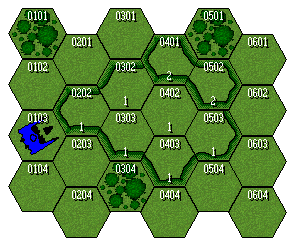
\includegraphics[width=7cm]{images/map2.png}
  % \caption{Trozo de mapa.}
\end{figure}

En nuestro ejemplo, los sucesores del nodo {\it 0103}, donde se encuentra
nuestro personaje, son: {\it 0102, 0202, 0203, 0104}

Ateniéndonos a las restricciones de {\it BattleTech}, vemos que
tenemos que tener en cuenta varias cosas:

\begin{itemize}
\item La diferencia de altura entre dos casillas colindantes no puede
  mayor a dos.
\item Si corremos, la profundidad del agua tiene que ser menor a uno.
\item En el caso de que andemos o corramos, debemos tener en cuenta si
  la casilla esta incendiada. En tal caso el fuego puede provocar un
  sobre calentamiento muy peligroso.
\item El el movimiento hacia atrás el máximo desnivel permitido es uno.
\end{itemize}

Para comprobar todos estos casos hacemos uso de la función {\bf
  checkCell(i,d, mov)}, donde {\bf i} es la casilla desde la que nos
queremos mover, {\bf d} es la casilla a la que nos queremos mover y {\bf mov} es
el tipo de movimiento a realizar.



\subsubsection{Función de evaluación}

\subsubsection{{\it \bf Función de coste}}

{\it PathFinder} también conoce el coste de cada movimiento ya que se
lo estamos diciendo en la función {\bf move\_cost}. Esta función nos
dice el coste real para movernos de un nodo a otro. \\

Para implementar esta función hemos tenido en cuenta varios factores:
\begin{itemize}
\item {\it El tipo de movimiento:} Andar, correr o saltar. Cada tipo de
  movimiento tiene sus propias restricciones, las cuales hemos de tener en
  cuenta.
\item {\it Los objetos.} Dependiendo del tipo de objeto(escombros, edificios ...) que se encuentre en una
  casilla, será más o menos costoso - o incluso imposible - el paso a través de
  ella.
\item {\it El nivel o profundiad} . El máximo   desnivel posible andando y
  corriendo es 2, mientras que saltando es un desnivel no mayor a los
  $PM_{salto}$.
\item {\it Tipo de terreno}. Cada tipo de terreno lleva asociado un coste distinto.
\item {\it Cambio de encaramiento}. Cambiar nuestro encaramiento también tiene
  un coste asociado, por lo tanto, debemos tener en cuenta el número de veces
  que giramos para poder desplazarnos a la casilla deseada.
\end{itemize}


\subsubsection{{\it \bf Función heurística}}

La última función que pasamos como argumento a {\it PathFinder} es
{\bf heuristic\_to\_goal}. Tal y como su nombre indica es la
heurística o coste del movimiento estimado para ir de un nodo origen a
un nodo destino.\\

Hay muchas formas de realizar esta función, la primera que utilizamos
es la {\bf distancia manhatan}.
$$ manhatan(x,y, x',y') = Vx + Vy $$
Siendo,
$$Vx = |x'-x| $$
$$Vy = |y'-y| $$

Esta heurística no es completamente precisa, ya que  nos ofrece una
sobreestimación del resultado correcto. Esto se debe a que la
conectividad entre celdas es diferente en un mapa hexagonal que en
uno rectangular, aunque la representación que hemos usado del mapa
pueda invitar al error, ya que usamos una matriz cuadrada.\\

Finalmente, tras realizar varios experimentos con la función {\it
  manhattan}, nos dimos cuenta de que conducía a resultados erróneos
en un número elevado de ocasiones. Así, encontramos la función que nos
da la distancia exacta para un tablero hexagonal:
$$ hexagonal\_distance(x,y, x',y') = Vx + max \{0, Vy- (Vx/2) -
factor\}  $$
Siendo:

$$ factor = \left \{ \begin{matrix} 0 & \mbox{if }mod(Vy,2) \ne 0 
    \\ mod(x-1,2) & \mbox{if } y < y'
    \\ mod(x'-1,2) & \mbox{otherwise } \end{matrix} \right. $$

De esta forma obtenemos la distancia real entre dos casillas de un tablero
hexagonal. Esto nos permite una mayor precisión en nuestros cálculos.

\subsubsection{Implementando la lista abierta}

Un aspecto interesante de implementación para mejorar la optimalidad
de nuestro programa es cómo implementar la lista de nodos
abiertos. Recordamos que A* usa la lista abierta para realizar un
seguimiento de los nodos que todavía tiene que vistar. Esta quizás sea
la estructura de datos más importante para el algoritmo, y su correcta
implementación es no trivial.\\

Aunque al principio empezamos con una implementación ineficiente de la
lista abierta, al decidir optimizar su implementación con una
estructura de datos más acertado mejoró cien veces su velocidad. Una
de las mejores fuentes de inspiración fueron las notas de
Amit.\ref{amit} \\

Combinando las colas de prioridad y las estructuras de datos tipo {\it
  set}, se consigue una cola de prioridad en la que sus componentes
están garantizados a ser únicos. \\

Esto nos proporciona una complejidad O(1) para pruebas de pertenencia,
y =(log N) para la extracción del menor elemento. La inserción en
cambio es mas complicada. Cuando un elemento no existe, se añade en
O(log N). En cambio, cuando ya existe, su prioridad se comprueba con
el nuevo elemento en O(1). Si la prioridad del nuevo elemento es
menor, se actualiza en la cola. Esto lleva un tiempo O(N).

\section{Módulo de Reacción}

El módulo de reacción es inmediatamente posterior al módulo de
movimiento. En esta fase se presenta la posibilidad de corregir el
encaramiento del torso para mejorar la estrategia de ataque -
mejorando el ángulo de disparo, tenemer a mas enemigos en línea de
visión, proteger partes débiles de nuestro mech, etc. -.\\

Las posibilidades que se nos presentan ahora son tres:
\begin{lstlisting}
  change = {0: 'Igual', 1: 'Derecha', 2:'Izquierda'}
\end{lstlisting}
Las cuales nos indican lois tres posibles cambios que podemos
realizar:
\begin{enumerate}
\item {\bf Igual}. Indica que no vamos a realizar ninguna
  cambio. Dejamos nuestro encaramiento intacto para la siguientes
  fases.
\item {\bf Derecha}. Giramos el mech para posicionar su torso una cara
  a Derecha.
\item {\bf Izquierda}.Giramos el mech para posicionar su torso una cara
  a Izquierda.
\end{enumerate}


\section{Módulo de Ataque con Armas}
\subsection{Lógica del ataque con armas}
El ataque con armas es una de las fases más importantes del juego.  El objetivo principal del Mech en la fase de ataque con armas será elegir a que enemigos y con que armas desea atacar.
Para poder realizar esta fase inteligentemente, dotaremos al Mech de la capacidad para analizar los distintos condicionantes que intervienen en el ataque. 
Antes de adentrarnos en que tipos de condicionantes, es necesario definir la estrategia general que realizarán nuestros Mechs. La estrategía será maximizar el daño sobre el atacado minimizando los daños en el atacante, es decir, atacaremos al Mech objetivo con todas las armas posibles mientras no se supere un valor umbral de daño en forma de calor en el atacante. 
Por tanto queda claro que los condicionantes que debe determinar el Mech serán:
\begin{enumerate}
\item Se realiza ataque.
\begin{enumerate}
\item Localización del Mech objetivo.
\item Elección de armas a usar en el ataque.
\end{enumerate}
\item No se realiza ataque.
\end{enumerate}
\subsection*{Se realiza un ataque}
En primer lugar es necesario saber si el Mech desea atacar o prefiero no realizar ningún tipo de ataque. Para discriminar entre las dos actuaciones nos basamos en calcular que enemigos están dentro de nuestra línea de visión, pero con la práctica, hemos visto que el programa \textit{LDVyC.exe} usado para calcular si un enemigo está en la línea de visión no funciona como esperabamos, es decir, el programa indica que un Mech está en linea de visión incluso cuando nuestro enemigo está a nuestra espalda. Por tanto, además de que esté en línea de visión, comprobamos que nuestro torso esté en un ángulo correcto para el ataque. Si existe al menos un Mech que cumpla estos requisitos el ataque se realizará. 

\subsubsection*{Localización del Mech objetivo}
Una vez seleccionados los Mechs que están dentro de nuestra línea de visión, elegimos cual es el que está más próximo a nosotros, calculando la distancia entre nuestra casilla en el tablero y las casillas de los enemigos a los que podemos atacar. Determinamos así el Mech objetivo sobre el que recaerán todo el poder de nuestras armas.

\subsubsection*{Elección de armas a usar en el ataque}
Para la resolución de este problema usaremos el enfoque teórico del algoritmo de la mochila que es del tipo algoritmo voraz. Lo algoritmos voraces son aquellos, que para resolver un determinado problema, sigue una metaheurística consistente en elegir la opción óptima en cada paso local con la esperanza de llegar a una solución general óptima.
\subsubsection*{Algoritmo de la mochila}
\begin{figure}[!h]
  \centering
  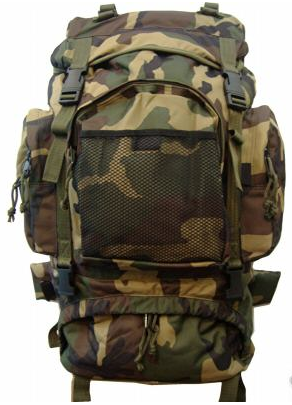
\includegraphics[width=10cm]{images/mochila.png}
  \caption{Algoritmo de la mochila}
\end{figure}
\begin{center}
\textit{“El problema de la mochila consiste en llenar una mochila con n objetos. Cada objeto $i$ tiene un peso determinado $ci$ siempre positivo y una utilidad o valor asociado, también positivo, $bi$. Se ha de considerar además que la mochila tiene una capacidad limitada $P$, por tanto, se han de escoger aquellos objetos $xi$ que maximicen la utilidad de quien llena la mochila sin exceder su capacidad”.}
\end{center}
Cada arma tiene un determinado valor equivalente a la distancia que es capaz de alcanzar en un disparo, por tanto bajo el enunciado del algoritmo de la mochila,  esos $n$ objetos a introducir en la mochila serán las armas que tiene el Mech que va a realizar el ataque, las cuales sean capaces de alcanzar al Mech objetivo. Una vez realizada esta discriminación en las armas a usar, determinaremos el peso de cada arma $ci$, que será la temperatura que genera en el arma sobre el Mech atacante al ser disparada. El parámetro $bi$ de calidad de cada arma $n$ responderá a la siguiente expresión:
$$ bi(n) = \frac{n.getDano()}{n.getCalor()}$$
La calidad de un arma será el resultado de dividir el daño que produce dicha arma en el atacado entre el calor que produce el arma en el atacante. Una vez ordenadas las armas en función de su calidad, debemos determinar la capacidad de la mochila $P$. Denominaremos a $P$ como el umbral máximo de temperatura que puede soportar un Mech después de realizar un ataque.
\subsubsection*{Determinación del valor umbral de temperatura}
Debe quedar claro que lanzar todas las armas posibles a nuestro enemigo no es una buena estrategia, ya que a cada disparo, la temperatura de nuestro Mech puede ascender de tal forma que incluso quede desactivado. Por tanto debemos calcular cuanta temperatura puede soportar el Mech en la realización del ataque. Sabemos que si un Mech pasa de 15º al acabar el turno, recibirá un punto de daño y si sobrepasa 26º recibirá dos. Por tanto podemos determinar el umbral de temperatura soportable de la siguiente forma:
\begin{itemize}
\item Si la temperatura del Mech es menor que 10º el umbral será 12º.
\item Si la temperatura del Mech está comprendida entre 10º y 15º el umbral será 9º.
\item Si la temperatura del Mech está comprendida entre 16º y 20º el umbral será 6º.
\item Si la temperatura del Mech está comprendida entre 20º y 26º el umbral será 4º.
\item Si la temperatura del Mech es mayor que 26º el umbral será 2º
\end{itemize}
Determinado $P$ (umbral de temperatura) ya tenemos las armas que usaremos en el ataque dentro de nuestra \textit{mochila}.
\subsection*{No se realiza ataque}
Si no hay ningún enemigo dentro de nuestra línea de visión no realizaremos ningún ataque, quedando como única posibilidad recoger un garrote, sí está alojado en nuestra casilla, para usarlo más tarde en un posible ataque físico.

\subsection*{Ataque físico}
Al igual que el ataque físico el Mech deberá tener en cuenta unos condicionantes para calcular la estrategia a seguir  durante la fase de ataques físicos:
\begin{enumerate}
\item Se realiza ataque.
\begin{enumerate}
\item Localización del Mech objetivo.
\item Elección de armas a usar en el ataque.
\end{enumerate}
\item No se realiza ataque.
\end{enumerate}
\subsection*{Se realiza ataque}
En primer lugar, al igual que en el ataque con armas, debemos conocer cuales son los posibles objetivos de dicho ataque. Para poder realizar un ataque físico es condición indispensable que el Mech atacado esté dentro de nuestra línea de visión, en un ángulo correcto para realizar el ataque, en una casilla adyacente y además que el nivel de su casilla sea igual a la nuestra. Si existe al menos un Mech enemigo que cumpla esos requisitos respecto a nuestro Mech se podrá realizar el ataque.
\subsubsection*{Localización del Mech objetivo}
A partir del conjunto de Mech objetivos que cumplan la condición para ser atacados, localizaremos el más cercano a nosotros y será el objetivo final de nuestro ataque físico.
\subsubsection*{Elección de las armas a usar en el ataque}
Determinado finalmente el Mech objetivo, necesitamos saber con que lo atacaremos. En el caso del ataque físico las armas a usar contra el objetivo serán nuestras extremidades, patadas y puñetazos, o un garrote recogido en anteriores fases.
Si disponemos del garrote, simplemente atacaremos con él, si no, procederemos a usar las extremidades. Para determinar que extremidades podemos usar en el ataque debemos  identificar cuales son las armas que usamos en el anterior ataque con armas, ya que si se ha usado un arma alojada en el brazo derecho, dicha extremidad ya no podrá ser usada en el ataque. Por tanto,  usando de nuevo el módulo de ataques con armas,  volveremos  a estimar  que armas fueron usada y en que extremidad  están  alojadas. Las extremidades que no fueron usadas en el ataque con armas podrán ser  utilizadas en el ataque físico. Si usamos los brazos debemos tener en cuenta que sólo se podrán usar los puños contra nuestro enemigo si no está tumbado en el suelo y si nuestro torso está en el ángulo correcto. De igual manera, si usamos las piernas,  el ángulo de ellas deberá ser correcto en relación al enemigo. Queda aclarar que si podemos usar las dos piernas, eligiremos una cualquiera, ya que no es posible dar una patada con dos piernas a la vez.
\subsection*{No se realiza ataque}
Si no se cumplen los requisitos para realizar un ataque físico el Mech no hará nada, pasando así a su fase de fin de turno.

\section{Final de Turno}

En esta fase es de utlidad para estar preparado para el siguiente turno de forma idónea. Podemos arrojar al suelo útiles de nuestro Mech, tales como munición o un garrote.
Además podremos apagar o encender radiadores, si disponemos de ellos, en función de nuestra temperatura.
Nuestro jugador inteligente arrojará el garrote si lo posee y si ha perdido alguna extremidad, buscará munición de las armas contenidas en las extremidades perdidas, arrojándolas al exterior.

\newpage
\renewcommand{\baselinestretch}{1}
\normalsize
\begin{thebibliography}{XXX}
\bibitem{0} González Duque, R., 2003. {\it ``PYTHON para todos.''} $1^{st}$ed. \\
\bibitem{2} Gutschmidt, Tom, 2003. {\it ``Game Programming with Python,
    Lua, and Ruby.''  } Premier Press \\
\bibitem{2} Weixiong Zhang, 1999. {\it ``State-Space Search. Algorithms,
    Complexity, Extensions and Applications.''} Springer-Verlag: NY \\
\bibitem{3} Pilgrim, Mark, 2004. {\it ``Dive into Python.''} Apress. \\
\bibitem{1} Amit Patel\\ \url{
    http://theory.stanford.edu/~amitp/GameProgramming/} \label{amit}
  \\
\bibitem{0} Russell, S. \& Norvig, P. {\it ``Artificial Intelligence: A
    Modern Approach''} $3^{rd}$ed. \\ \label{russell}
\bibitem{4}  \url{http://www.policyalmanac.org/games/aStarTutorial.htm}\\
\bibitem{5}  \url{http://www.solaris7.com/ }\\
\bibitem{6}  \url{ }\\
\bibitem{7}  \url{http://code.google.com/p/smart-player/ } \label{googlecode}
\end{thebibliography}

\end{document}
